
\section{A Primer on Lithium-Ion Battery Chemistries and Degradation}

The effectiveness, safety, and economic viability of any V2G strategy remain fundamentally constrained by the physical and chemical characteristics of vehicle batteries. Battery chemistry selection dictates EV operational envelopes, influencing energy density, power capabilities, lifespan, and safety profiles. Clear understanding of these trade-offs proves essential for developing robust, realistic, and responsible control algorithms.
\subsection{Fundamental Concepts and Degradation Mechanisms}
Battery degradation is a complex and irreversible process that gradually reduces a cell’s ability to store and deliver energy. It manifests primarily as capacity loss (energy fade) and as an increase in internal resistance (power fade). These phenomena are usually attributed to two categories of mechanisms: \textit{calendar aging} and \textit{cyclic aging} \cite{birkl2017degradation}.
\noindent   
\\
\textbf{Calendar aging} occurs while the battery is at rest, regardless of whether it is fully charged or nearly empty. The main mechanism behind this process is the slow growth of the \textbf{Solid Electrolyte Interphase (SEI)} layer on the graphite anode. While a thin and stable SEI layer is necessary for battery operation, its continuous thickening consumes both active lithium and electrolyte, resulting in irreversible capacity loss. The rate of SEI growth is particularly sensitive to operating conditions. High temperatures accelerate chemical reaction rates, including parasitic ones, making storage in hot environments detrimental. Similarly, high states of charge (SoC) correspond to low anode potentials, which increase the reactivity of graphite with the electrolyte and foster faster SEI growth \cite{vetter2005ageing}. For this reason, leaving electric vehicles stored for long periods at 100\% SoC is generally discouraged.
\noindent   
\\
\textbf{Cyclic aging}, in contrast, results from the processes that take place during charging and discharging. This form of degradation is of particular importance for V2G applications, which inherently involve frequent cycling. Several mechanisms contribute to cyclic aging. The repeated intercalation and de-intercalation of lithium ions induce mechanical stress due to the expansion and contraction of electrode materials. Over time, this stress may generate micro-cracks in electrode particles, leading to a loss of electrical contact and a reduction of active material, effects that become more severe with larger \textbf{Depths of Discharge (DoD)}. Mechanical volume changes can also compromise the integrity of the SEI layer, causing cracks that expose fresh anode surface to the electrolyte and trigger renewed SEI growth. In addition, under demanding conditions,such as very high charging rates (high C-rates) or low temperatures,lithium ions may deposit as metallic lithium on the anode surface rather than intercalating properly. This phenomenon, known as lithium plating, is particularly harmful: it leads to rapid capacity loss and may produce dendritic structures capable of piercing the separator, thereby creating internal short circuits and serious safety hazards \cite{birkl2017degradation}.
\noindent   
\\
Both calendar and cyclic aging are unavoidable, the latter is especially critical for V2G systems. Since these applications require frequent and sometimes deep cycling, understanding and mitigating cyclic degradation is paramount to guarantee long-term system viability.


\subsection{Key Automotive Chemistries}

The EV market is dominated by several key lithium-ion battery families, primarily distinguished by cathode materials. Each chemistry presents different balances of performance characteristics.

\begin{itemize}
    \item \textbf{Lithium Nickel Manganese Cobalt Oxide (NMC):} For years, this has been the most popular choice due to its excellent balance of energy density, power, and cycle life. The ratio of Nickel, Manganese, and Cobalt can be adjusted (such as NMC111, NMC532, NMC811) to prioritize either energy density (high Nickel) or safety and longevity (lower Nickel).
    
    \item \textbf{Lithium Nickel Cobalt Aluminum Oxide (NCA):} Offers very high specific energy (energy density by weight), enabling longer vehicle range. However, it typically comes at the cost of slightly lower cycle life and narrower safety margins compared to NMC, requiring more sophisticated thermal management.
    
    \item \textbf{Lithium Iron Phosphate (LFP):} Is rapidly gaining market share, particularly in standard-range vehicles, due to lower cost (no cobalt, an expensive and ethically contentious material) and superior safety. LFP batteries offer exceptional cycle life (often 3-4 times that of NMC/NCA) and are considered the safest common Li-ion chemistry due to high thermal stability. Their main drawback involves lower energy density.
    
    \item \textbf{Lithium Titanate Oxide (LTO):} This represents a more niche chemistry using titanate-based anodes instead of graphite. This provides exceptional safety (virtually no thermal runaway risk), extremely long cycle life (>10,000 cycles), and excellent low-temperature performance. However, very low energy density and high cost currently limit its use to specialized applications.
\end{itemize}

\subsection{Voltage Profiles and the Challenge of SoC Estimation}

The relationship between battery open-circuit voltage and SoC represents a critical, non-linear function unique to each chemistry. The derivative of cell voltage with respect to DoD, $\frac{dV_{cell}}{d(DoD)}$, constitutes a key parameter for Battery Management Systems (BMS). Steep, monotonic slopes allow BMS to accurately infer SoC from simple voltage measurements. Conversely, flat slopes make this estimation extremely difficult.

\begin{figure}[H]
    \centering
    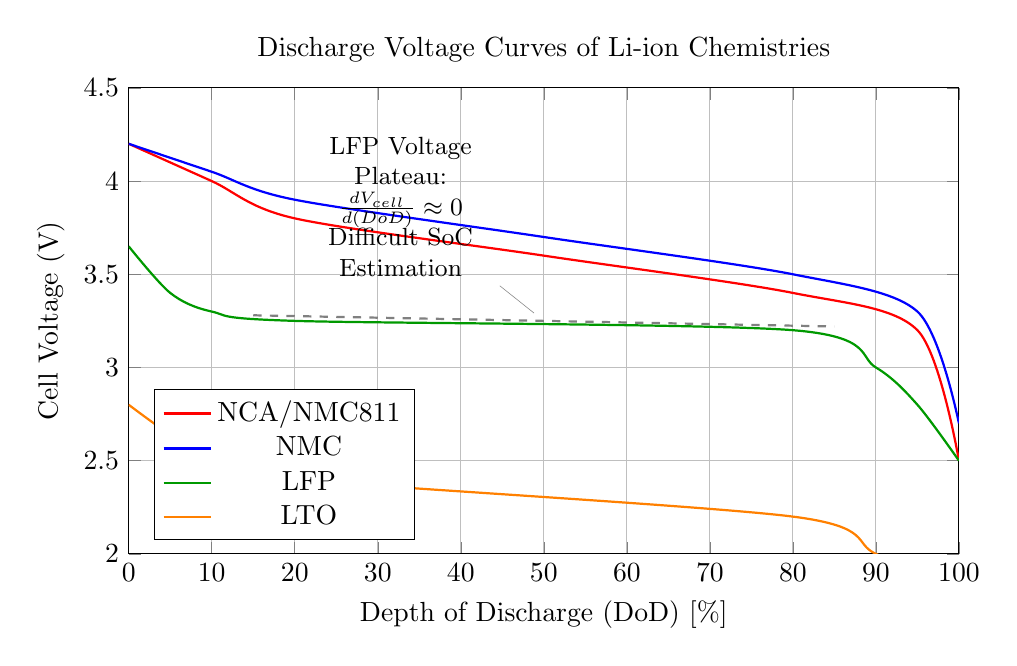
\begin{tikzpicture}
        \begin{axis}[
            title={Discharge Voltage Curves of Li-ion Chemistries},
            xlabel={Depth of Discharge (DoD) [\%]},
            ylabel={Cell Voltage (V)},
            xmin=0, xmax=100,
            ymin=2.0, ymax=4.5,
            grid=major,
            legend pos=south west,
            width=\textwidth,
            height=7.5cm,
        ]
        \addplot[smooth, thick, red] coordinates { (0, 4.2) (10, 4.0) (20, 3.8) (50, 3.6) (80, 3.4) (95, 3.2) (100, 2.5) };
        \addlegendentry{NCA/NMC811}

        \addplot[smooth, thick, blue] coordinates { (0, 4.2) (10, 4.05) (20, 3.9) (50, 3.7) (80, 3.5) (95, 3.3) (100, 2.7) };
        \addlegendentry{NMC}

        \addplot[smooth, thick, green!60!black] coordinates { (0, 3.65) (5, 3.4) (10, 3.3) (20, 3.25) (80, 3.2) (90, 3.0) (95, 2.8) (100, 2.5) };
        \addlegendentry{LFP}
        
        \addplot[smooth, thick, orange] coordinates { (0, 2.8) (10, 2.5) (20, 2.4) (80, 2.2) (90, 2.0) (100, 1.8) };
        \addlegendentry{LTO}

        \draw[dashed, thick, gray] (axis cs:15,3.28) -- (axis cs:85,3.22);
        \node[pin=135:{\parbox{2.5cm}{\centering \small LFP Voltage Plateau: \\ $\frac{dV_{cell}}{d(DoD)} \approx 0$ \\ Difficult SoC Estimation}}] at (axis cs:50,3.25) {};
        \end{axis}
    \end{tikzpicture}
    \caption{Typical discharge voltage curves for various lithium-ion chemistries. The extremely flat profile of LFP makes accurate SoC estimation challenging based on voltage alone, necessitating more complex estimation techniques like Coulomb counting and periodic recalibration.}
    \label{fig:voltage_curves_detailed}
\end{figure}
\noindent
As shown in Figure \ref{fig:voltage_curves_detailed}, LFP's remarkably flat voltage plateau makes it nearly impossible for BMS to determine precise SoC in the central operating range (from approximately 20\% to 80\%) using voltage alone. This necessitates more complex estimation techniques, such as Coulomb counting (integrating current over time), which can suffer from drift. To correct this drift, LFP-equipped vehicles require periodic full charges to 100\% for BMS recalibration. This represents an important operational constraint that V2G control strategies must consider.

\subsection{Comparative Analysis and Safety Considerations}

The trade-offs between chemistries are summarized in Table \ref{tab:chem_comparison_detailed}. Safety remains paramount, with the primary risk being thermal runaway,a dangerous, self-sustaining exothermic reaction. This risk relates directly to cathode material chemical and thermal stability. Higher energy density generally means more energy packed into smaller mass, which can be released violently if cells are compromised. Consequently, critical temperatures for initiating thermal runaway are generally lower for higher energy density chemistries. LFP's stable phosphate-based structure makes it far more resistant to thermal runaway than nickel-based counterparts, a key reason for its growing popularity.

\begin{table}[H]
\centering
\small
\caption{Comparative analysis of key automotive battery chemistries, highlighting the trade-offs between performance and safety.}
\label{tab:chem_comparison_detailed}
\begin{tabularx}{\textwidth}{
  @{}
  >{\bfseries\RaggedRight}X
  *{5}{>{\centering\arraybackslash}X}
  @{}
}
\toprule
Metric & NCA & NMC & LFP & LTO & LCO \\
\midrule
Energy Density (Wh/kg) & 200 - 260 (Highest) & 150 - 220 (High) & 90 - 160 (Moderate) & 60 - 110 (Low) & 150-200 (High) \\
\addlinespace
Cycle Life & 1000 - 2000 & 1000 - 2500 & 2000 - 5000+ & $>$10,000 & 500 - 1000 \\
\addlinespace
Safety & Good & Very Good & Excellent & Excellent & Poor \\
\addlinespace
Thermal Runaway Temp ($^{\circ}$C) & $\sim$150 - 180 & $\sim$180 - 210 & $\sim$220 - 270 & $>$ 250 & $\sim$150 \\
\bottomrule
\end{tabularx}
\end{table}